\section{Datová struktura stránky}

Kdyby byl celý web tvořen jen vizuálními prvky, moc by toho nedělal. O vizuálním stavu stránky se špatně píše, protože většinou stačí pro dosažení cílového vzhledu jen naskládat několik komponent na sebe. To zajímavé, co sice normální uživatel nevidí, ale bez čeho by stránka nefungovala, je její datová část. Díky ní můžete reprezentovat, jaká mají prvky data, jak jsou propojené, a jak spolu celá architektura funguje.

\subsection{MobX store a validace dat}
Jak funguje MobX už víte. Asi vás proto nepřekvapí, že svůj vlastní store má každá z již vyjmenovaných stránek. Díky tomu nemusím používat useState() a kazit si tak svá data Reactem.

Store stránek je třída složená z polí obsahujících všechna data, která se budou na stránce používat, jejich náležitých getterů (a většinou i setterů) a konstruktoru. Všechna pole, která se mění, musí být označena dekorátorem @observable a jejich změna musí být obalená buďto v runInAction() funkci nebo @action dekorátoru.

Konstruktor by měl správně jen dosadit základní hodnoty, spustit nějaké interní funkce a zavolat makeObservable(this), čímž aktivuje MobX. Externí data z API by ho mohly zbrzdit nebo vyvolat vyjímku, proto by si je měl vývojář zavolat sám. Proto má každá ze stránek svoji veřejně přístupnou metodu init(), která se v Reactu volá po prvním renderu. Tím ovšem vzniká další problém – když se stránka načte, ještě nemá data. Proto jsem si vytvořil vlastní funkci load(), kterou všechny stránky používají, spolu s isInitialized stavem. Ten se změní, jakmile se všechna data načtou, a díky tomu vím, kdy stránku zobrazit uživateli, a kdy ji nahradit načítací animací.

Každý ze storů má dvě speciální pole. FormChanged se nastaví na true po tom, co změníte jakákoliv data na stránce – třeba vlastní přezdívku. Tím se Vám zároveň odemkne tlačítko s odesláním dat, čímž jsem alespoň částečně zabránil tomu, aby náš server zaplňovaly prázdné požadavky. Jakmile data odešlete, formChanged se opět nastaví na false a tlačítko zamkne.

FormLoading se zase nastaví na true po tom, co data uložíte. Zamkne všechna pole, aby hodnoty zůstaly během odesílání konzistentní, a zůstane tak, dokud server nepošle odpověď.

Pokud je na stránkách potřeba nějaké volání na API, i to naleznete zde. Kromě metody init() a save(), které jsou všude, mají některé stránky i své vlastní metody – třeba na smazání a nahrání fotky v nastavení účtu, nebo připojení Facebooku a Instagramu v sociálních sítích.

U nastavení účtu a změny hesla jsem se nevyhnul ani validaci dat. Pokaždé, když kliknete na tlačítko pro uložení, spustí se metoda validate(). Ta aktualizuje hodnoty jako nicknameIsValid, nebo emailIsValid podle toho, zda nejsou prázdné nebo v neplatném formátu. Getterem isValid() se dá následně zjistit, zda validace prošla.

Pokud bylo vráceno true, spustí se část, kterou mají všechny stránky stejnou – funkce save(). Podobně jako load() bere jako argument metodu, kterou má spustit (každý store má kromě init() i svůj save()), a také již zmíněné formLoading a formChanged, se kterými podle odpovědi serveru manipuluje. Ať už je odpověď jakákoliv, vždy se dole zobrazí Toast, díky němuž uživatel zjistí, zda se operace zdařila, server neodpovídá, nebo se například neshodují hesla.
\newpage
\subsection{Data, konvertory a API}
Postupně se dostávám výš a výš v naší frontendové hierarchii. Všechna data, která jsem dostával ve storu, jsou vlastně jen datové třídy. Konkrétně se jedná o třídy s definovanými poli reprezentujícími jejich obsah, gettery, a konstruktorem, jehož jediný parametr je interface se všemi dosaditelnými hodnotami, kterým třídu můžeme naplnit. Protože nemá settery, jde to jen jednorázově, a tak veškeré změny proměnných řeší až store a já zde nemusím používat MobX a @observable dekorátory.

Zhruba na stejné úrovni jako data mohou být i konvertory. Ne vždy jsou totiž data z databáze v pro nás ideálním formátu. Například čas i enumy jsou vyjádřené jako string, s čímž se ale špatně pracuje a museli bychom ho před každým použitím převést. Stejné je to i s různými objekty. Konverze probíhá ještě před tím, než se vše vloží do datové třídy, takže na stránce dostávám takovou strukturu dat, se kterou už můžu jednoduše pracovat. Přenos zpátky probíhá podobným způsobem, jen je třeba data zase převést na serverem podporovaný formát.

Ještě výš se nachází námi zpracované metody pro práci s API. Jsou systematicky rozdělené do několika tříd podle místa použití, abych, pokud potřebuji pracovat s nastavením, nemusel importovat něco, co má navíc funkce pro získání nejnovějších cest, přihlášení uživatele, a vrácení posledních hodnocení na Googlu. Každá metoda přijímá kromě dat také parametr na úpravu požadavku, díky kterému můžu měnit jeho hlavičku, cookie, nebo zda chci, aby při chybě stránka nespadla, a já si tak mohl vyjímku odchytit sám.

Každá z metod nakonec zavolá funkci importovanou z api.ts souboru. Tento soubor o délce přes čtyřicet tisíc řádků se automaticky generuje pomocí nástroje Swagger, a skrývá reálnou API implementaci, která je vlastně jen soubor všech možných HTTP požadavků, které fungují jako most mezi frontendem a backendem. Výš už pro mě cesta nevede.

Ve Storybooku je struktura trochu odlišná. API funkce se volají stále stejně, ale při načtení jakékoliv story se jejich původní implementace přepíší na mock. Ten vrací mock datové třídy, díky čemuž nejsou potřeba žádné konvertory. Abychom alespoň částečně simulovali internetovou odezvu, každá z metod vrací data až po uplynutí doby 300 milisekund.
\newpage
\subsection{Unit testy}
Abychom si byli jistí, že web funguje správně alespoň po datové stránce, máme pomocí Jestu (a dříve Karmy) napsaných několik stovek testů. Všechny jsou ve složce test, která má úplně stejnou strukturu jako složka s komponentami, jen s tím rozdílem, že všechny soubory mají příponu .spec.ts.

Každá datová část se testuje trochu jinak. Aktuálně nejvýše v hierarchii jsou testy na datové třídy. Protože jsou neměnné a dají se naplnit jen jednou, je potřeba jen vyzkoušet, zda se data dosadila správně. To jde zjistit pomocí tvorby falešných dat, jejich dosazením a následně porovnáním všech veřejných getterů.

Testům se samozřejmě nevyhnou ani konvertory. Zde konkrétně byl potřeba jen jeden, a to pro první stránku s uživatelským nastavením. Testy jsou z principu podobné těm datovým, opět jen stačí vytvořit falešná data, ty dát do konvertoru, a pak zkontrolovat data nového objektu, který od něj dostaneme.

Poslední a největší skupina testů se zaměřuje na samotné komponenty a jejich MobX store. Zároveň jsou také nejkomplexnější, protože musí pokrýt všechno od přidávání a získávání dat, validací a komunikací s API.

Stejně jako u ostatních typů se i tady kontroluje dosazení do konstruktoru a následný stav. Kromě toho se ale proměnné zkouší nastavit již mimo konstruktor a zkoumají, zda správně funguje setter. Na všech stránkách se ve většině setterů nastavoval i formChanged parametr, který byl také potřeba do testů zahrnout.

Validace už je docela komplikovaná. Například u přezdívky se jen stačilo ujistit, že není prázdná. Email už zase musel mít správnou strukturu. A AppearAs, Combo box, který určoval, zda budete viditelní pod přezdívkou nebo pod jménem, si musel být jistý, že při výběru „Pod jménem“ byla správně nastavená alespoň jednu část jména a „Pod přezdívkou“ zase požadoval nastavenou přezdívku, která se validovala v předchozím kroku.

Následně se testují všechny metody integrující API volání. Ačkoliv jsou všechny z nich jen mocky a ve skutečnosti na server nevolají, můžu vyzkoušet, zda se pod nimi zabalená API metoda zavolala s těmi parametry, které jsem jejímu rodiči předal. K tomu se výborně hodí SpyObject.
\newpage
\subsection{Architektura webu}
Pro lepší představu o funkci webu vám nyní vysvětlím, co všechno se stane, pokud stránku navštívíte.

Vše začne zadáním adresy \href{https://www.worldee.com}{worldee.com} do adresního řádku (1). Požadavek se odešle na náš Next.js server, kde si ho jako první převezme middleware. Ten zkontroluje a případně upraví cookies a hlavičky požadavku a do url přidá lokalizaci. Potom ho předá routeru, který podle url najde většinou již předkreslenou požadovanou stránku, přeloží ji a posílá zpátky do prohlížeče (2).

Pokud byla stránka předem předkreslená, uživatel už nyní může vidět všechny její prvky, ač jde zatím jen o vizuál postrádají jakoukoliv funkčnost. Pokud ne, stránka je prázdná. Prohlížeč musí spustit React (3), stránku inicializovat a podle odpovědi serveru vytvořit všechny kompozice a komponenty. Po prvním renderu začíná probíhat komunikace s naším PHP serverem (4) a získaná data jsou z JSONu převáděna na použitelný formát (5), kterým jsou plněny datové třídy. Stránka je nyní plně načtená, celý proces trval jednotky sekund. 

\begin{figure}[!h]
    \centering
    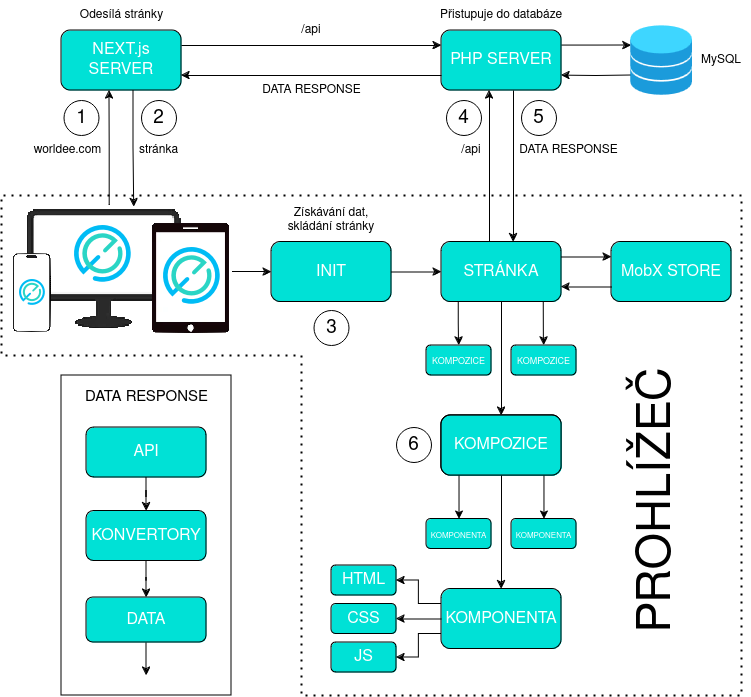
\includegraphics[width=1\linewidth]{obrazky/architektura.png}
    \caption{Diagram architektury webu. Zdroj: vlastní práce.}
\end{figure}
\clearpage


\newpage